\textbf{\underline{OZ 9 - Wisselstroomkringen - Oefening 1:}}
\vspace{0.5cm}

Bereken $Z$, $X_L$, $X_C$ en $\phi$ voor een AC-circuit met $R = 300 \ \Omega$, $C = 11.0 \ \mu\text{F}$, $L = 0,200 \ \text{H}$, en $f = (500/\pi) \ \text{Hz}$. Teken het bijhorende fasordiagram.

% \begin{enumerate}[(a)]
%     \item #
% \end{enumerate}

\begin{description}[labelwidth=1.5cm, leftmargin=!]
    \item[Geg. :]  $R = 300 \ \Omega$, $C = 11.0 \ \mu\text{F}$, $L = 0,200 \ \text{H}$, $f = (500/\pi) \ \text{Hz}$ 
    \item[Gevr. :] $Z$, $X_L$, $X_C$, $\phi$ ?
    \item[Opl. :]   
        We berekenen $\omega$:
        \begin{equation*}
            \omega = 2\pi f = 1000 \ \text{rad/s}
        \end{equation*}
        We berekenen $X_L$ en $X_C$:
        \begin{align*}
            X_L &= \omega L \approx 200 \ \Omega \\ X_C &= \frac{1}{\omega C} \approx 90.9 \ \Omega
        \end{align*}
        \begin{itemize}
            \item Serieschakeling: $I$ is gelijk. We hebben het volgende fasor diagram
                \begin{center}
                    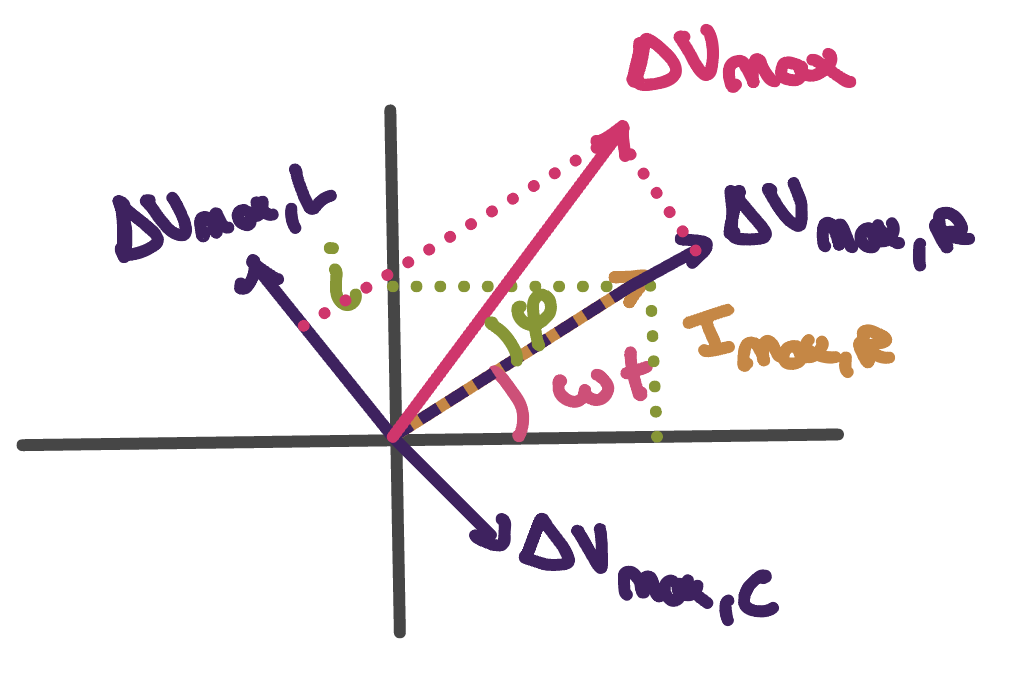
\includegraphics[scale=0.3]{oz09/resources/Oz9Oef1-serie.png}
                \end{center}
                waarbij 
                \begin{equation*}
                    |\Delta V_{\text{max},R}| \approx \frac{3}{2}|\Delta V_{\text{max},L}| \approx 3|\Delta V_{\text{max},C}|.
                \end{equation*}
                We berekenen $Z$ (met Pythagoras):
                \begin{equation*}
                    Z = \sqrt{R^2 + (X_L - X_C)^2} \approx 319 \ \Omega
                \end{equation*}
                We berekenen $\phi$:
                \begin{equation*}
                    \phi = \tan^{-1}\left(\frac{X_L - X_C}{R}\right) \approx 20^\circ
                \end{equation*}
  
            \item Parallelschakeling: $\Delta V$ is gelijk. We hebben het volgende fasor diagram
                \begin{center}
                    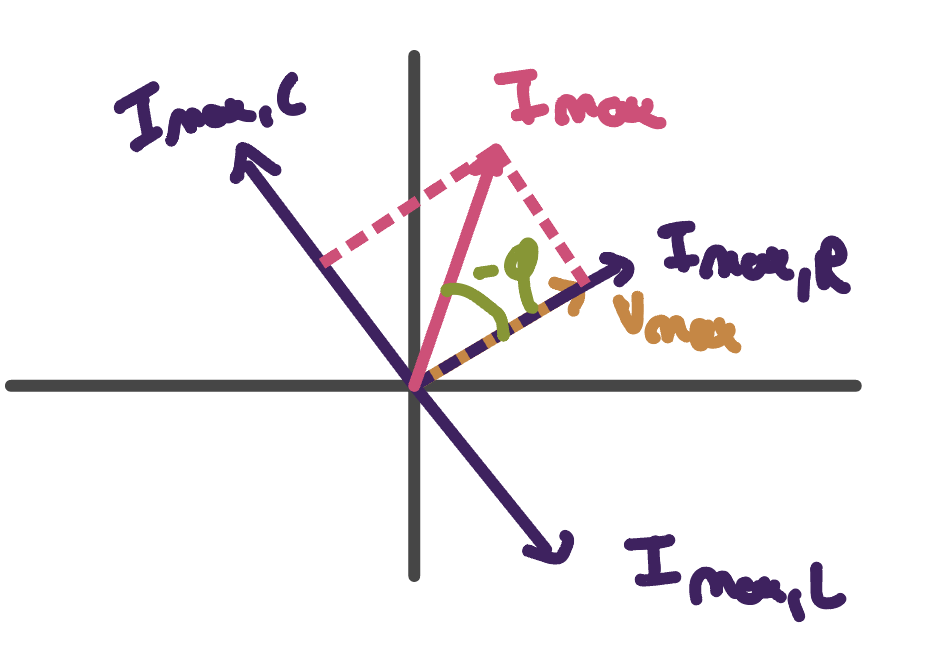
\includegraphics[scale=0.3]{oz09/resources/Oz9Oef1-parallel.png}
                \end{center}
                waarbij
                \begin{equation*}
                    |\Delta I_{\text{max},C}| \approx \frac{2}{3}|\Delta I_{\text{max},L}| \approx 3|\Delta I_{\text{max},R}|.
                \end{equation*}
                We berekenen $Z$ (met Pythagoras):
                \begin{equation*}
                    Z = \frac{1}{\sqrt{\frac{1}{R^2} + \left(\frac{1}{X_L} - \frac{1}{X_C}\right)^2}} = 103 \ \Omega
                \end{equation*}
                We berekenen $\phi$:
                \begin{equation*}
                    \phi = \tan^{-1}\left(\frac{\frac{1}{X_L} - \frac{1}{X_R}}{\frac{1}{R}}\right) \approx -61^\circ
                \end{equation*}
        \end{itemize}
\end{description}

\vspace{1cm}